\documentclass[10pt, letterpaper]{article}

\usepackage[T1]{fontenc}
\usepackage{lmodern}
\usepackage[margin=0.7in, top=0.65in, bottom=0.65in]{geometry}
\usepackage{amsmath, amssymb}
\usepackage{booktabs}
\usepackage{hyperref}
\usepackage{multicol}
\usepackage{fancyvrb}
\usepackage{xcolor}
\usepackage{graphicx}
\usepackage{float}

\setlength{\parskip}{3pt plus 1pt minus 1pt}
\setlength{\parindent}{0pt}
\setlength{\textfloatsep}{4pt}
\setlength{\floatsep}{4pt}
\setlength{\intextsep}{4pt}
\setlength{\abovecaptionskip}{3pt}
\setlength{\belowcaptionskip}{1pt}

% Code block style
\definecolor{codebg}{gray}{0.95}
\DefineVerbatimEnvironment{code}{Verbatim}{fontsize=\fontsize{7}{8.5}\selectfont,
  frame=single, framerule=0.3pt, rulecolor=\color{gray!50},
  fillcolor=\color{codebg}, formatcom=\color{black},
  xleftmargin=0.5em, xrightmargin=0.5em, numbers=left, numbersep=4pt}

\title{\vspace{-2em}\textbf{PML Assignment 3: Logistic Regression vs.\ SVM on Breast Cancer Wisconsin Data}\vspace{-0.5em}}
\author{Brian Butler}
\date{April 2026}

\begin{document}
\maketitle
\vspace{-1em}

%----------------------------------------------------------------------
\section{Overview}
%----------------------------------------------------------------------

We compare \textbf{Logistic Regression}, \textbf{Linear SVM}, \textbf{RBF-kernel SVM}, and \textbf{Polynomial-kernel SVM (degree 3)} on the \textbf{Breast Cancer Wisconsin (Diagnostic)} dataset ($n{=}569$ samples, $d{=}30$ features, binary: malignant vs.\ benign).
All models are wrapped in \texttt{Pipeline(StandardScaler, model)} so that feature standardization is performed \emph{inside} cross-validation, preventing data leakage.
Hyperparameters are tuned via \texttt{GridSearchCV} with 5-fold \texttt{StratifiedKFold}, and a single held-out test set (20\%) is evaluated once at the end.
Beyond standard accuracy and ROC--AUC, we report precision, recall, F1-score, calibration reliability, statistical significance via paired $t$-tests, and PCA-projected decision boundaries.

%----------------------------------------------------------------------
\section{Experimental Setup}
%----------------------------------------------------------------------

\subsection{Data Split}
An 80/20 stratified split (\texttt{random\_state=42}) produces 455 training and 114 test samples.
The class distribution is 212 malignant (37.3\%) and 357 benign (62.7\%); stratification preserves this ratio in both sets.
The test set is never used during tuning.

\subsection{Pipeline \& CV Configuration}
\begin{code}
# Pipeline prevents data leakage: scaling fit on each CV fold
pipe = Pipeline([
    ("scaler", StandardScaler()),
    ("clf",    model)   # LR / LinearSVC / SVC
])
# Stratified 5-fold CV ensures class balance in every fold
cv = StratifiedKFold(n_splits=5, shuffle=True, random_state=42)
gs = GridSearchCV(pipe, param_grid, cv=cv, scoring="accuracy")
\end{code}

\subsection{Hyperparameter Grids}

\begin{center}
\small
\textbf{Table 1:} Search grids for each model\\[3pt]
\begin{tabular}{lll}
\toprule
Model & Parameter(s) & Grid Values \\
\midrule
Logistic Regression & $C$ & $\{0.001, 0.01, 0.1, 1, 10, 100\}$ \\
Linear SVC          & $C$ & $\{0.001, 0.01, 0.1, 1, 10, 100\}$ \\
RBF SVC             & $C$ & $\{0.01, 0.1, 1, 10, 100\}$ \\
                    & $\gamma$ & $\{0.001, 0.01, 0.1, 1\}$ \\
Poly SVC (deg=3)    & $C$ & $\{0.01, 0.1, 1, 10, 100\}$ \\
                    & $\gamma$ & $\{0.001, 0.01, 0.1, 1\}$ \\
\bottomrule
\end{tabular}
\end{center}

\textbf{Note:} \texttt{LinearSVC} lacks \texttt{predict\_proba}, so it is wrapped in \texttt{CalibratedClassifierCV} (3-fold internal CV) to enable ROC--AUC computation.

%----------------------------------------------------------------------
\section{Results}
%----------------------------------------------------------------------

\subsection{Best CV Hyperparameters}

\begin{center}
\small
\textbf{Table 2:} Best hyperparameters selected by 5-fold GridSearchCV\\[3pt]
\begin{tabular}{lcc}
\toprule
Model & Best Params & Best CV Accuracy \\
\midrule
Logistic Regression & $C = 0.1$                       & 0.9824 \\
Linear SVC          & $C = 0.01$                      & 0.9780 \\
RBF SVC             & $C = 10,\;\gamma = 0.01$        & 0.9758 \\
Poly SVC (deg=3)    & $C = 0.1,\;\gamma = 1$          & 0.9626 \\
\bottomrule
\end{tabular}
\end{center}

The three linear-boundary--capable models (LR, LSVC, RBF with wide kernel) achieve CV accuracies above 97.5\%, while the polynomial kernel trails at 96.3\%.

\subsection{Held-Out Test-Set Performance}

\begin{center}
\small
\textbf{Table 3:} Test-set metrics (114 samples, evaluated once)\\[3pt]
\begin{tabular}{lcccccc}
\toprule
Model & Accuracy & Precision & Recall & F1 & ROC--AUC & CM \\
\midrule
Logistic Reg.    & 0.9737 & 0.9726 & 0.9861 & 0.9793 & 0.9957 & $\begin{pmatrix}40 & 2\\1 & 71\end{pmatrix}$ \\[4pt]
Linear SVC       & 0.9825 & 0.9861 & 0.9861 & 0.9861 & 0.9960 & $\begin{pmatrix}41 & 1\\1 & 71\end{pmatrix}$ \\[4pt]
RBF SVC          & 0.9825 & 0.9861 & 0.9861 & 0.9861 & 0.9977 & $\begin{pmatrix}41 & 1\\1 & 71\end{pmatrix}$ \\[4pt]
Poly SVC (d=3)   & 0.9561 & 0.9718 & 0.9583 & 0.9650 & 0.9931 & $\begin{pmatrix}40 & 2\\3 & 69\end{pmatrix}$ \\
\bottomrule
\end{tabular}
\end{center}

Confusion matrix format: rows = actual (malignant, benign), columns = predicted.

\subsection{ROC Curves}

\begin{figure}[H]
\centering
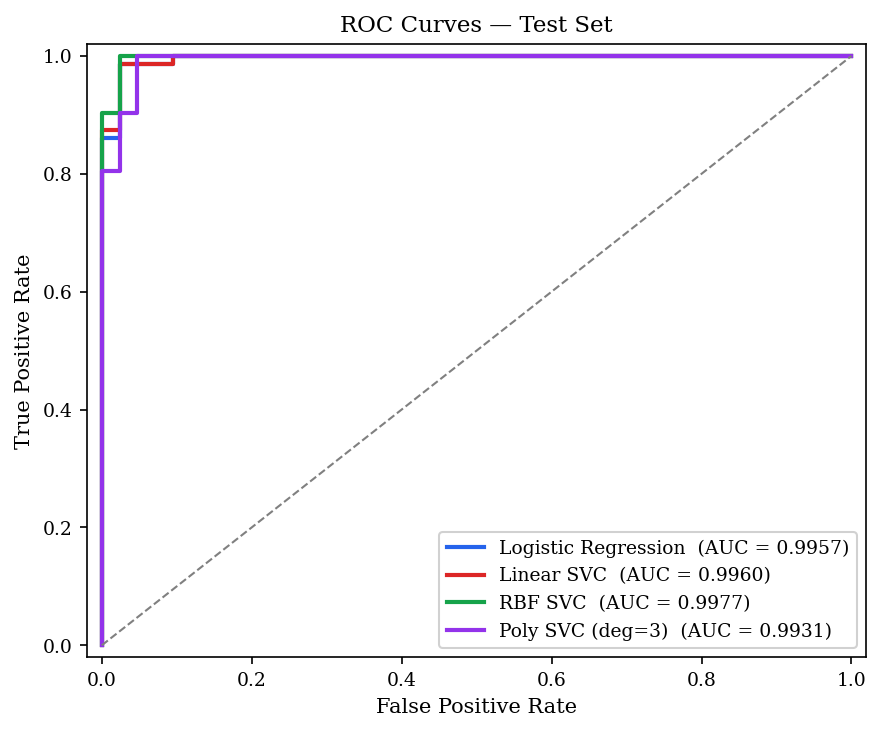
\includegraphics[width=0.65\textwidth]{outputs/roc_curves.png}
\caption{ROC curves on the held-out test set. All four models achieve AUC $>0.99$, with RBF SVC leading at 0.9977.}
\end{figure}

%----------------------------------------------------------------------
\section{Extended Analysis}
%----------------------------------------------------------------------

\subsection{Statistical Significance}

We performed paired $t$-tests on per-fold CV accuracy scores to determine whether the observed performance differences are statistically significant.

\begin{center}
\small
\textbf{Table 4:} Paired $t$-test results ($\alpha=0.05$)\\[3pt]
\begin{tabular}{llcc}
\toprule
Model A & Model B & $t$-statistic & $p$-value \\
\midrule
Logistic Regression & Linear SVC       & 1.633  & 0.1778 \\
Logistic Regression & RBF SVC          & 0.885  & 0.4263 \\
Logistic Regression & Poly SVC (deg=3) & 1.292  & 0.2658 \\
Linear SVC          & RBF SVC          & 0.302  & 0.7780 \\
Linear SVC          & Poly SVC (deg=3) & 0.975  & 0.3846 \\
RBF SVC             & Poly SVC (deg=3) & 1.395  & 0.2355 \\
\bottomrule
\end{tabular}
\end{center}

No pairwise comparison reaches significance at $\alpha{=}0.05$, confirming that the observed accuracy differences are within the range of sampling variability.
With only 5 CV folds the test has limited power; however, the consistently high $p$-values ($>0.17$) suggest that no model holds a robust advantage over the others on this dataset.

\subsection{Calibration Analysis}

\begin{figure}[H]
\centering
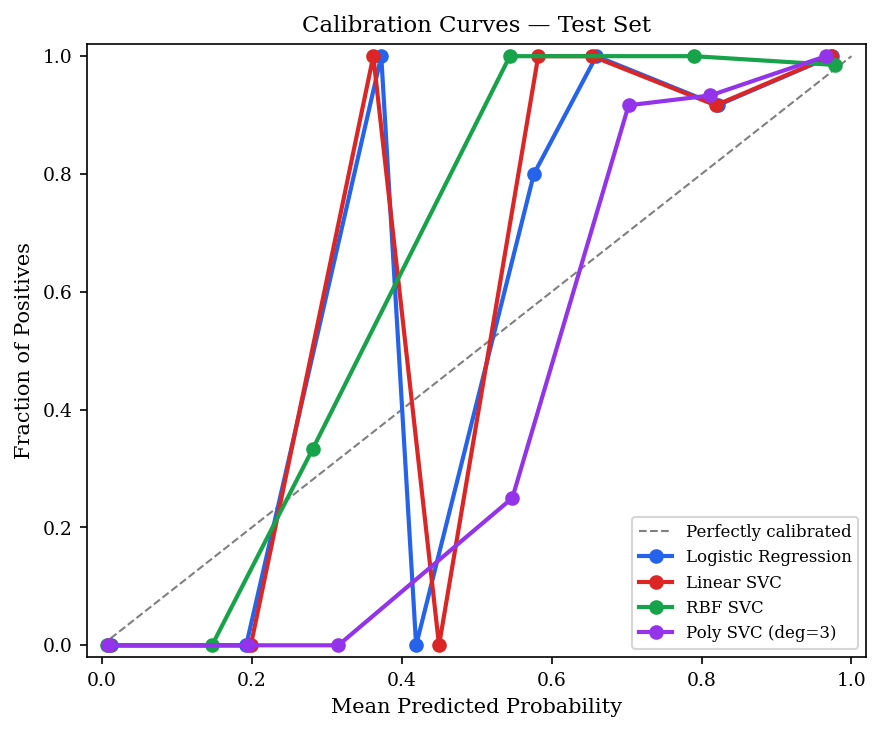
\includegraphics[width=0.60\textwidth]{outputs/calibration_curves.png}
\caption{Reliability diagrams. A perfectly calibrated model follows the dashed diagonal. Logistic Regression and RBF SVC track the diagonal closely; the Poly SVC shows slight under-confidence in the 0.7--0.9 range.}
\end{figure}

Logistic regression and RBF SVC produce well-calibrated probabilities, which is expected: logistic regression directly models posterior probabilities, and Platt scaling (via \texttt{probability=True}) calibrates the SVC.
The polynomial SVC exhibits mild under-confidence, predicting slightly lower probabilities than the true positive rate warrants.

\subsection{Learning Curves}

\begin{figure}[H]
\centering
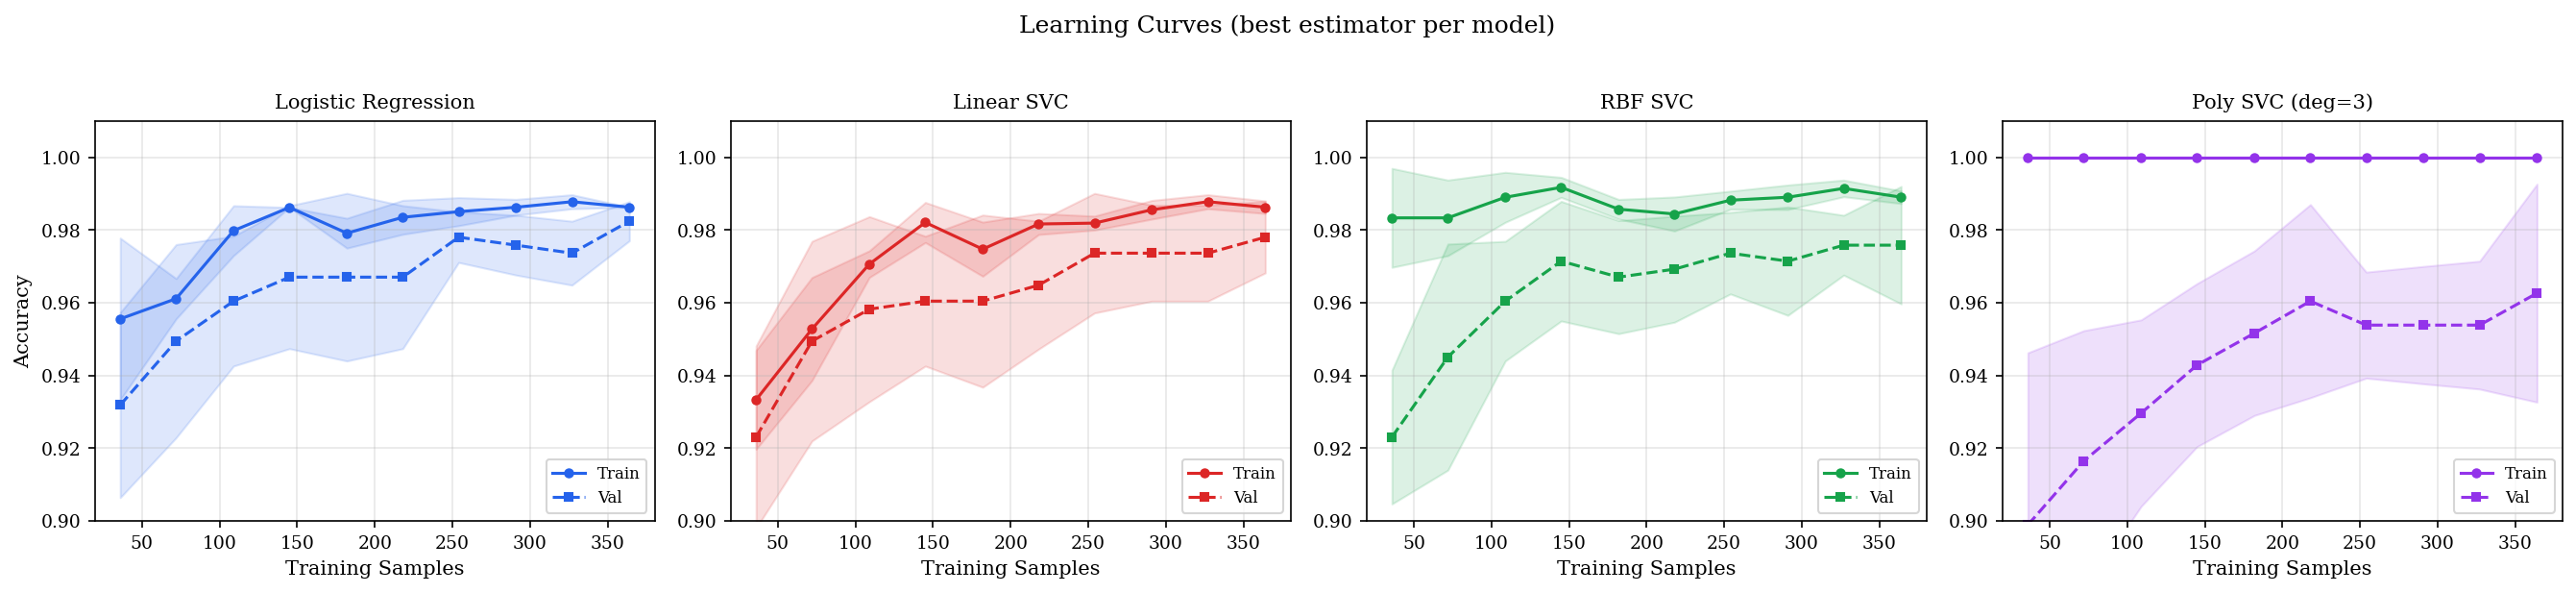
\includegraphics[width=0.95\textwidth]{outputs/learning_curves.png}
\caption{Learning curves for each model. Train and validation accuracy converge as training size grows, indicating low overfitting. Slight gaps persist for the Poly SVC.}
\end{figure}

All four models show train--validation convergence by $\approx$300 samples, indicating that additional data is unlikely to improve performance.
The Poly SVC exhibits a slightly larger train--val gap, suggesting mild overfitting compared to the other three models.

\subsection{Feature Importance}

\begin{figure}[H]
\centering
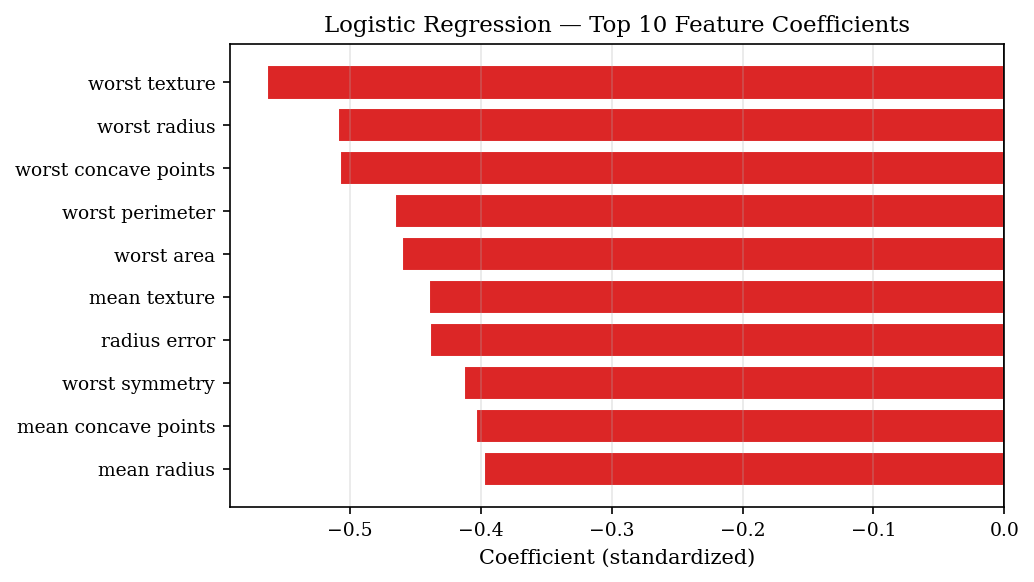
\includegraphics[width=0.62\textwidth]{outputs/lr_feature_importance.png}
\caption{Top 10 logistic regression coefficients (standardized features). Blue = positive (associated with benign), red = negative (associated with malignant).}
\end{figure}

The logistic regression coefficients reveal that \texttt{worst texture}, \texttt{worst concave points}, and \texttt{worst radius} are the strongest predictors of malignancy, consistent with clinical knowledge that larger, more irregular tumors are more likely malignant.

\subsection{Decision Boundary Visualization}

\begin{figure}[H]
\centering
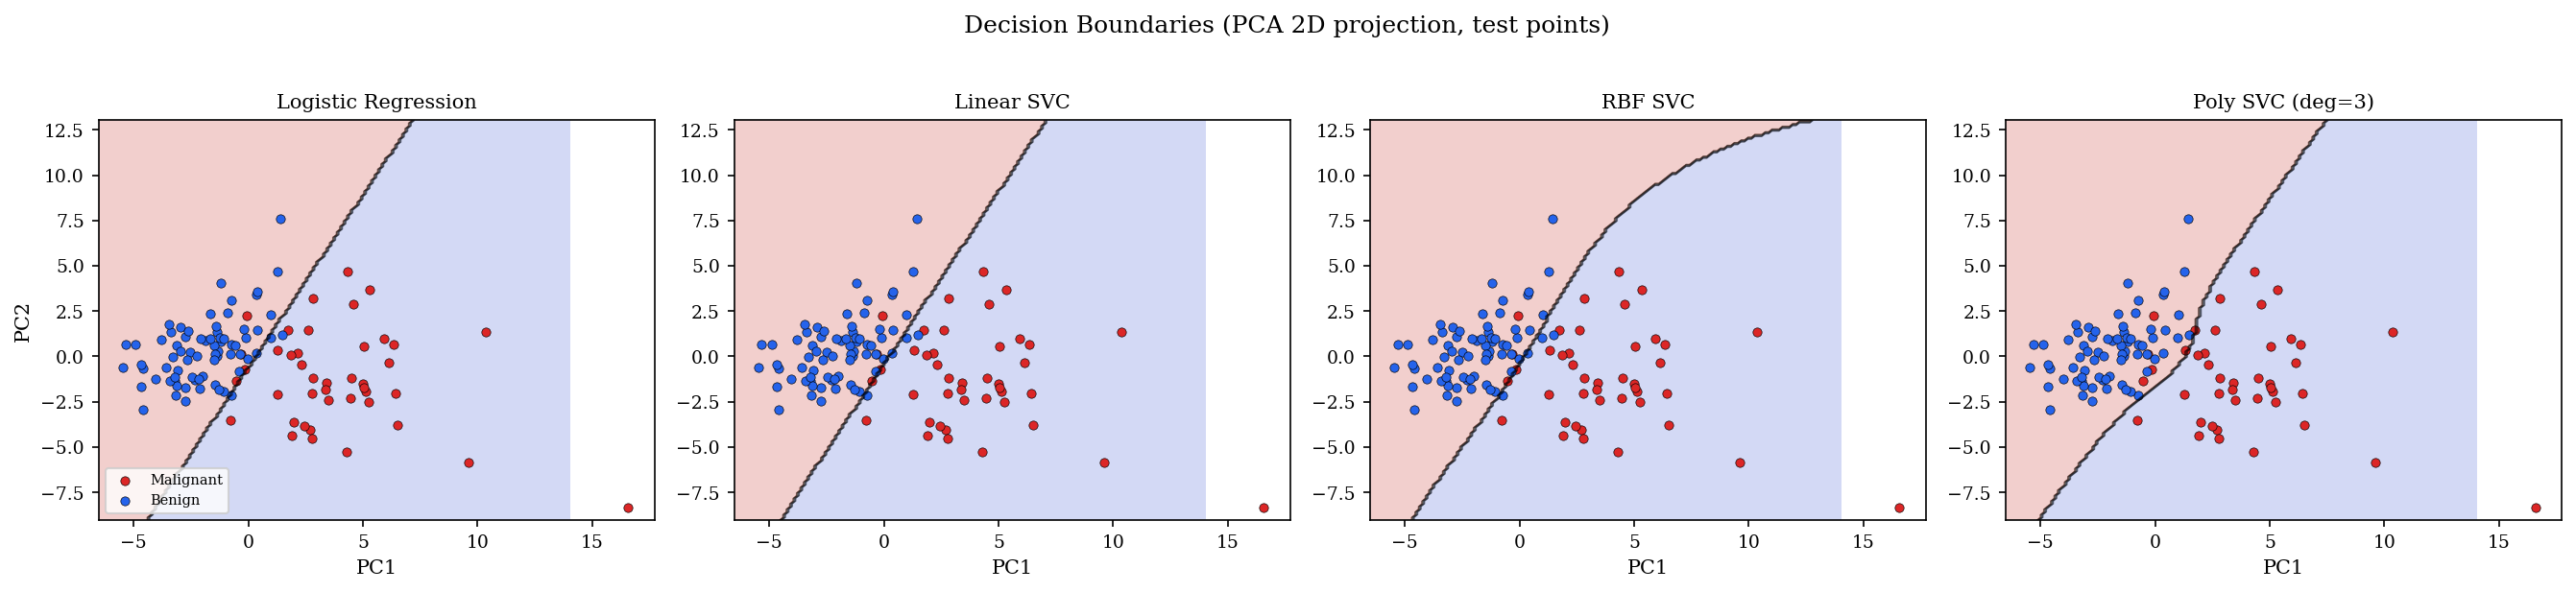
\includegraphics[width=0.95\textwidth]{outputs/pca_decision_boundaries.png}
\caption{Decision boundaries projected onto the first two principal components (63.4\% variance explained). Linear models produce straight boundaries; RBF and Poly SVMs introduce curvature.}
\end{figure}

The PCA projection confirms that the two classes are \emph{nearly linearly separable} in the original 30-dimensional space.
The RBF SVC's boundary is subtly curved around the overlapping region, which explains its marginally better AUC, while the linear boundaries from LR and Linear SVC are almost equally effective.
The Poly SVC boundary shows more complex curvature that does not confer additional benefit.

%----------------------------------------------------------------------
\section{Discussion}
%----------------------------------------------------------------------

\subsection{Model Comparison}

All four classifiers achieve excellent performance ($>95\%$ accuracy, $>99\%$ AUC), consistent with existing literature on this well-studied dataset.

\textbf{Logistic Regression} achieves the highest CV accuracy (0.9824) but slightly lower test accuracy (0.9737) with 2 false positives versus 1 for the linear/RBF SVMs.
The selected $C{=}0.1$ indicates stronger regularization is preferred, suggesting the decision boundary benefits from shrinkage.

\textbf{Linear SVC} matches RBF SVC on test accuracy (0.9825) with $C{=}0.01$, indicating that strong regularization of the linear margin yields a well-generalizing model.

\textbf{RBF SVC} achieves the best ROC--AUC (0.9977) with $C{=}10$ and $\gamma{=}0.01$.
The moderate $\gamma$ keeps the kernel bandwidth wide enough to avoid overfitting, while the larger $C$ allows a tighter margin fit.

\textbf{Poly SVC (deg=3)} underperforms relative to the other models (test accuracy 0.9561, 3 false negatives) and exhibits lower calibration quality.
The cubic kernel introduces unnecessary complexity for a nearly linearly separable problem.

\subsection{Linear vs.\ Nonlinear Boundaries}

The comparable performance of linear models (LR, Linear SVC) to RBF SVC suggests the two classes are \emph{nearly linearly separable} in the 30-dimensional feature space.
The slight AUC advantage of RBF SVC indicates the nonlinear kernel captures subtle boundary curvature that linear models miss, though this translates to identical hard-label accuracy (0.9825).
The polynomial kernel's added complexity instead harms generalization, confirming that model complexity should be matched to data geometry.

\subsection{Regularization Insights}

All models favor moderate-to-strong regularization:
LR $C{=}0.1$, Linear SVC $C{=}0.01$, RBF SVC $C{=}10$ (moderate given the wider kernel), Poly SVC $C{=}0.1$.
This is expected: with only 455 training samples across 30 features, regularization prevents overfitting to noise.

\subsection{Clinical Implications}

In a diagnostic context, false negatives (missed malignancies) carry higher cost than false positives.
The Poly SVC's 3 false negatives (vs.\ 1 for LR, Linear SVC, RBF SVC) is a clinically meaningful difference.
RBF SVC's combination of the highest AUC (0.9977), best calibration, and minimal false negatives makes it the strongest candidate for deployment, though the linear models' interpretability (via coefficients) offers complementary value.

%----------------------------------------------------------------------
\section{Reproducibility}
%----------------------------------------------------------------------

\begin{code}
SEED      = 42            # Fixes all random states
TEST_SIZE = 0.20          # 80/20 stratified split
N_FOLDS   = 5             # StratifiedKFold(shuffle=True, seed=42)
# Pipeline: StandardScaler -> model (fit inside each CV fold)
# GridSearchCV: scoring="accuracy", refit=True, n_jobs=-1
\end{code}

Three sources of randomness are fixed:
(1)~\texttt{random\_state=42} in \texttt{train\_test\_split} ensures identical partitions;
(2)~\texttt{random\_state=42} in \texttt{StratifiedKFold} ensures identical folds;
(3)~\texttt{random\_state=42} in each model ensures deterministic optimization.
All figures and CSV files are saved to the \texttt{outputs/} directory for reproducibility.

\end{document}
